% Created 2025-01-11 Sat 08:09
% Intended LaTeX compiler: pdflatex
\documentclass[11pt]{article}
\usepackage[utf8]{inputenc}
\usepackage[T1]{fontenc}
\usepackage{graphicx}
\usepackage{longtable}
\usepackage{wrapfig}
\usepackage{rotating}
\usepackage[normalem]{ulem}
\usepackage{amsmath}
\usepackage{amssymb}
\usepackage{capt-of}
\usepackage{hyperref}
\usepackage{tikz}
\usepackage[paperwidth=14.58in, paperheight=10.42in, margin=0.1in]{geometry}
\pagestyle{empty}
\date{}
\title{Neural Network Diagram}
\hypersetup{
 pdfauthor={},
 pdftitle={Neural Network Diagram},
 pdfkeywords={},
 pdfsubject={},
 pdfcreator={Emacs 29.4 (Org mode 9.7.12)}, 
 pdflang={English}}
\begin{document}

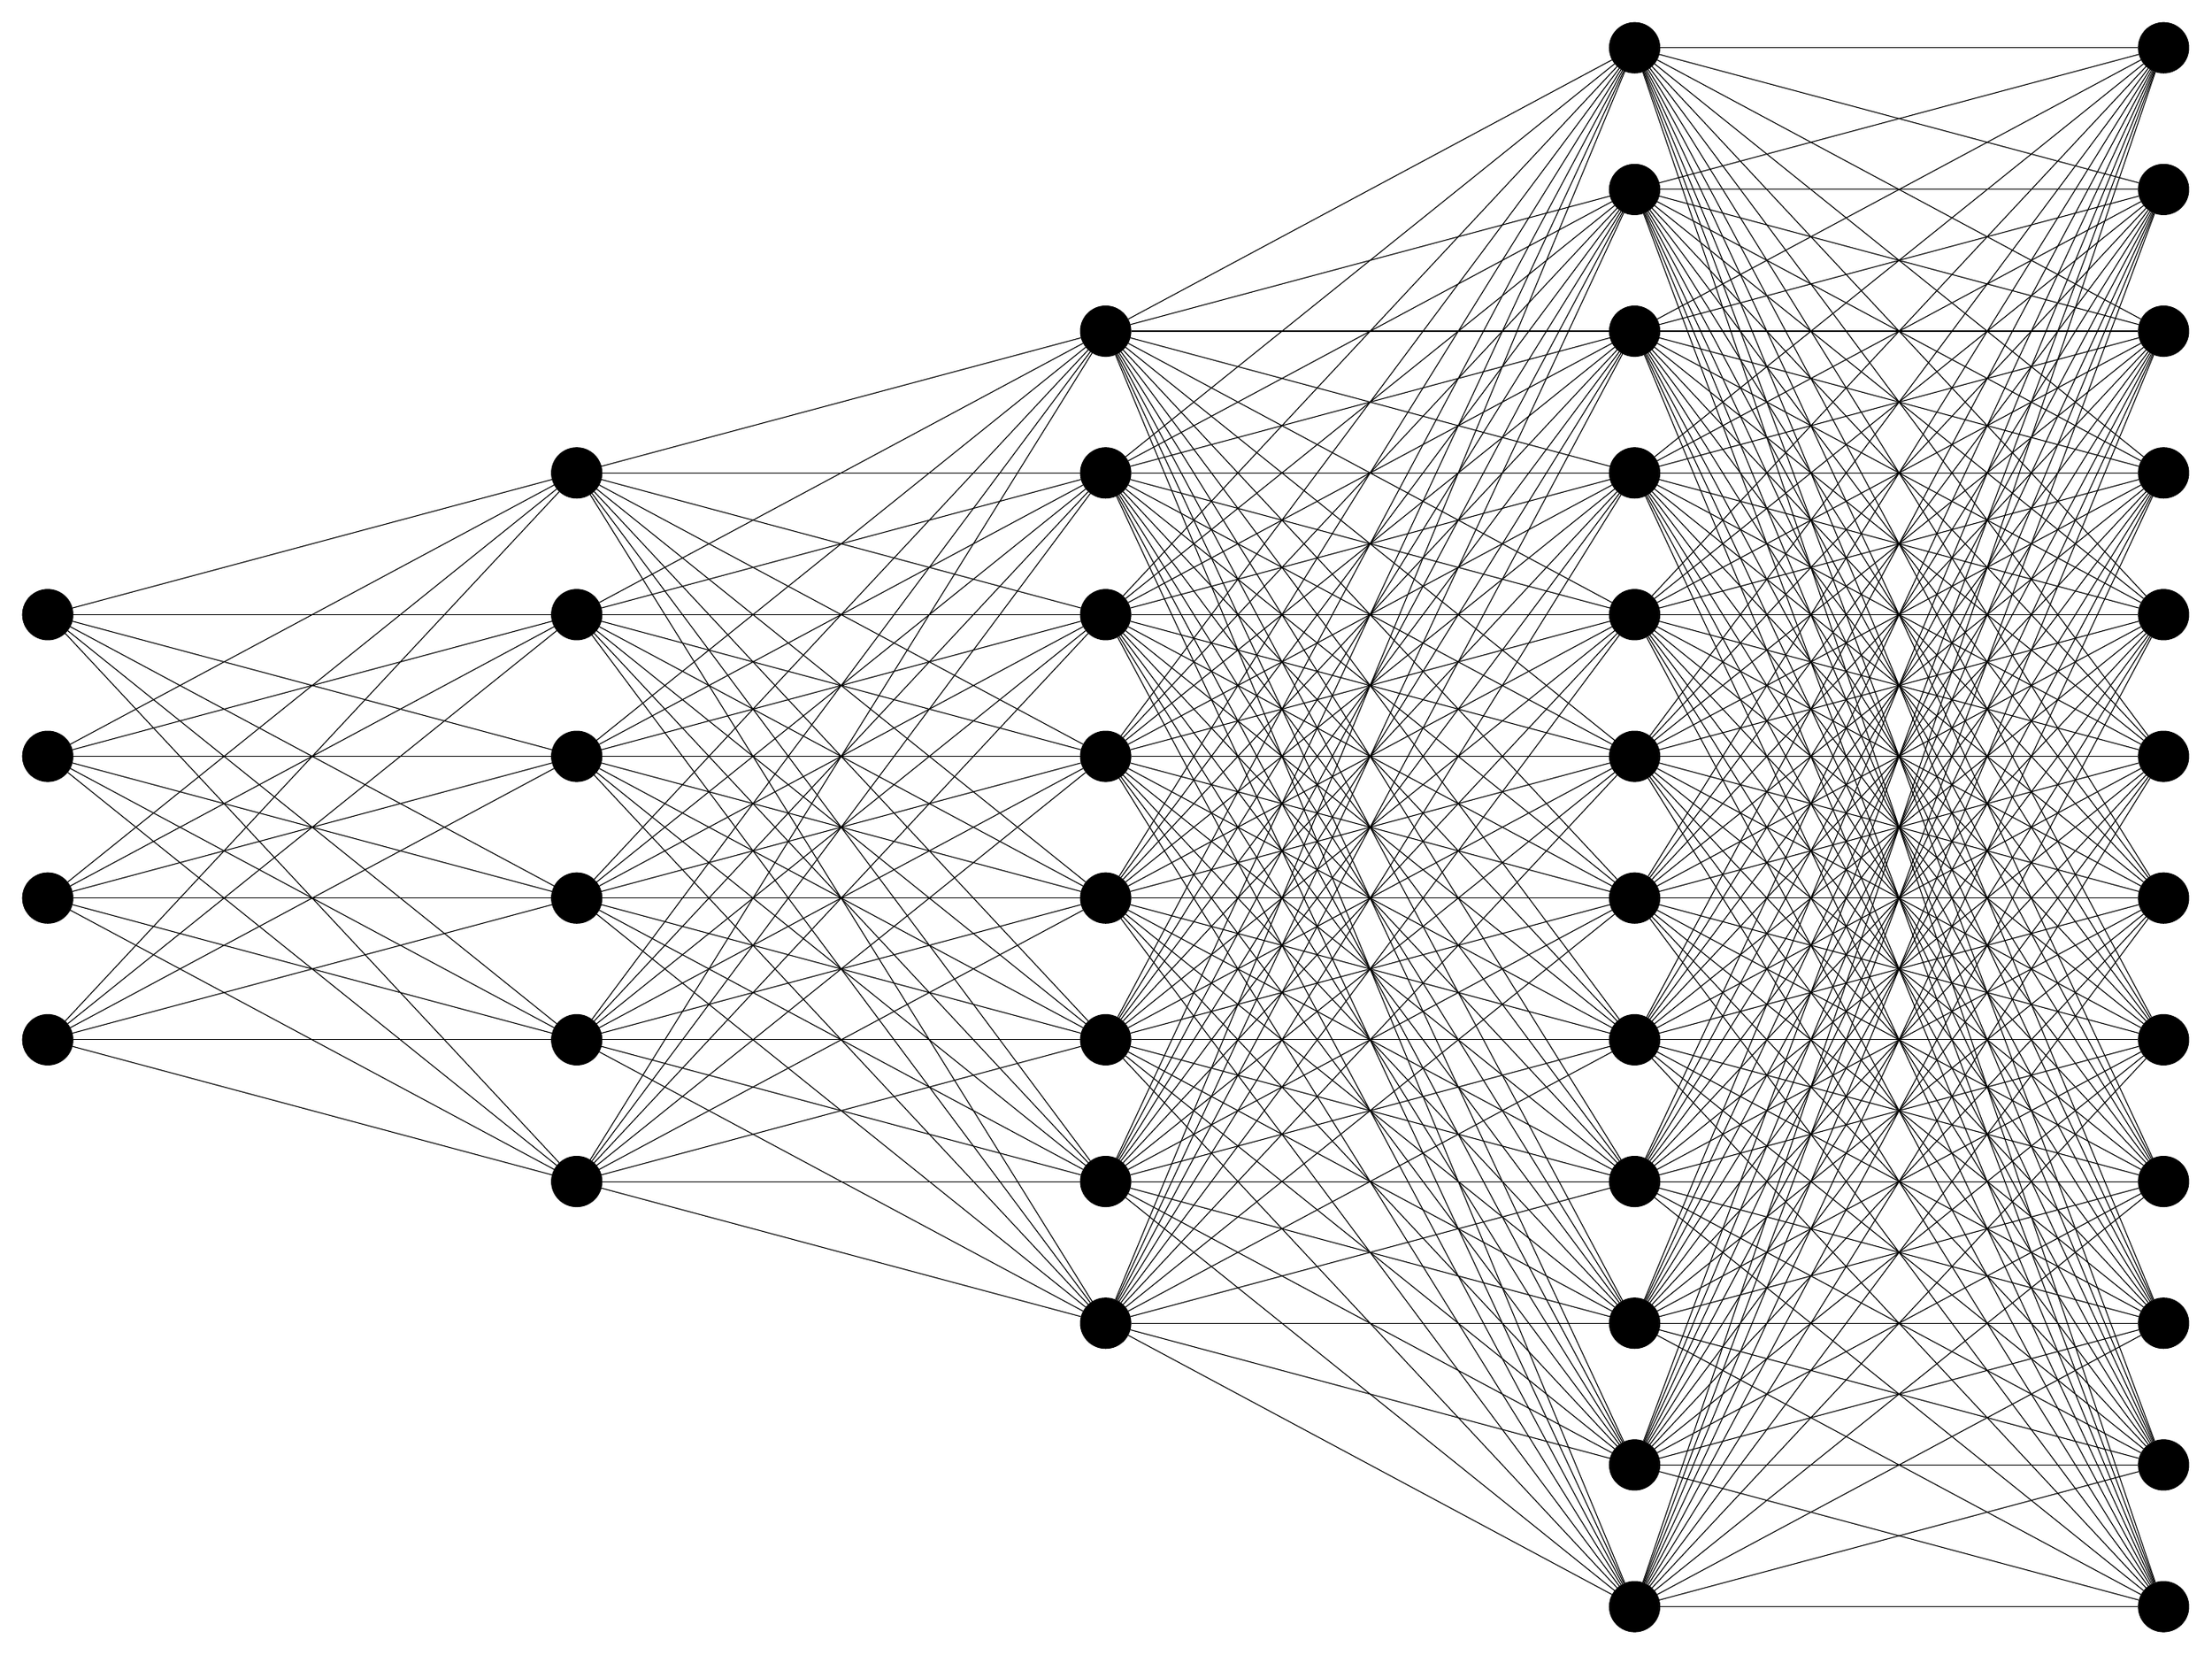
\begin{tikzpicture}[every node/.style={circle, draw,fill=black, minimum size=0.8cm}, node distance=2cm]

% Define a variable for spacing
\def\spacing{2.25}
\def\hspacing{2.8}

% Input layer (4 neurons)
\foreach \i in {1,...,4} {
    \node (input\i) at (\hspacing*0, {\spacing*1 - \spacing * \i}) {};
}

% First hidden layer (6 neurons)
\foreach \i in {1,...,6} {
    \node (h1_\i) at (\hspacing*3, {\spacing*2 - \spacing * \i}) {};
}

% Second hidden layer (8 neurons)
\foreach \i in {1,...,8} {
    \node (h2_\i) at (\hspacing*6, {\spacing*3 - \spacing * \i}) {};
}

% Third hidden layer (12 neurons)
\foreach \i in {1,...,12} {
    \node (h3_\i) at (\hspacing*9, {\spacing*5 - \spacing* \i}) {};
}

% Fourth hidden layer (12 neurons)
\foreach \i in {1,...,12} {
    \node (h4_\i) at (\hspacing*12, {\spacing*5 - \spacing * \i}) {};
}

% Connections from input to first hidden layer
\foreach \i in {1,...,4} {
    \foreach \j in {1,...,6} {
        \draw[-] (input\i) -- (h1_\j);
    }
}

% Connections from first hidden to second hidden layer
\foreach \i in {1,...,6} {
    \foreach \j in {1,...,8} {
        \draw[-] (h1_\i) -- (h2_\j);
    }
}

% Connections from second hidden to third hidden layer
\foreach \i in {1,...,8} {
    \foreach \j in {1,...,12} {
        \draw[-] (h2_\i) -- (h3_\j);
    }
}

% Connections from third hidden to fourth hidden layer
\foreach \i in {1,...,12} {
    \foreach \j in {1,...,12} {
        \draw[-] (h3_\i) -- (h4_\j);
    }
}

\end{tikzpicture}
\end{document}
